\graphicspath{{Figures/}}
\chapter{Commande Robuste par Mode Glissant} \label{chap:robust control}
Dans les Chapitres~\ref{chap:introduction_Gen} et~\ref{chap:optimal control}, on a vu que l'on peut commander un système linéaire de la forme de~\eqref{eq-chap2:syslin_commande} par une commande qui a la forme d'un retour d'état linéaire $\command = -\matriceK\state$. En l'occurence, les gains $\matriceK$ sont calculés soit par la méthode de placement des pôles, ou bien par la minimisation d'une fonction-coût quadratique. Par ailleurs, on a vu que les systèmes nonlinéaires de la forme de~\eqref{eq-chap1:generic nnlinear sys} peuvent être stabilisés en choisissant une commande $\command = \gamma(\state)$, potentiellement nonlinéaires, tel que le système en boucle fermée $\stateDot = f\left(\state,\gamma(\state)\right)$ est asymptotiquement stable.  En particulier  dans le Chapitre~\ref{chap:backstepping}, on a étudié la méthode dite de Backstepping qui permet de synthétiser une loi de commande de manière systèmatique en se basant sur le $2^\text{ème}$ théorème de Lyapunov (Théorème~\ref{thm:direct lyapunov method}). 

Les lois de commande vu jusqu'à maintenant ont des propriétés en commun : 
\begin{itemize}
	\item Continues par rapport à l'état,
	\item Gains constants,
	\item Synthèse de la commande dépend du modèle du système (notamment pour les systèmes nonlinéaires).
\end{itemize}
Dans ce cas, on dit que le système en boucle fermée est à \emph{structure unique}. Cependant en partique, certains systèmes échappent à cette classification. 
\section{Systèmes à Structure Variable}
Certains régulateurs de température fonctionnement en mode ‘on/off’ sur la base d'une logique dite en  hystéresis. La loi de commande générée commute entre deux valeurs distinctes et elle est donc discontinues. Ce cas de figure n'est pas isolé. En effet dans l'industrie automobile, le système de freinage Anti Blocking System (ABS) se base sur un concept similaire : effectuer des coups de frein discontinus et rapides afin de ralentir éfficacement la vitesse du véhicule tout en évitant le blocage des roues et le glissement. La commande de la vitesse des moteurs à courant continu s'éffectue pratiquement aussi par un signal sous forme d'impulsion dont la largeur est modulée (Pulse Width Modulation (PWM)). Dans le domaine de l'avionique, le pilote automatique ne garde pas des paramtres constant tout au long du vol, mais change de paramètres en fonction des différents phases de vol. Cette opération est connu sous le nom  de la commande à gains pré-programmés (gains-scheduling control) : un ensemble de commande est pré-implémenté pour chaque point de fonctionnement par lequel l'avion vas (ou peut) passer durant le vol. Ensuite, le régulateur commute entre les différents lois de commande (moyennant une interpoloation pour limiter les discontinuités) sur la base du changement des certains paramètres de vol, comme l'altitude.  

Dans tout ces exemples, le régulateur change de structure (formulation) ou bien de paramètres suivant une certaine logique de commutation, et par conséquent le système en boucle fermée devient à \emph{structure variable}.
\subsection{Avantages des systèmes à structure variable}
Avoir un système à structure variable peut présenter plusieurs avantages. En effet, on peut combiner les avantages de chaque système en terme de stabilité, rapidité, précision, etc. En particulier, on peut bénéficier de nouvelles propriétés qui sont non inhérentes de chacun des systèmes considérés séparément. En effet, soit le système linéaire suivant :
\begin{equation}\label{eq-chap4:expl linear system VSS}
	\stateDot = \begin{bmatrix}
		0&1\\0&1
	\end{bmatrix}\state + \begin{bmatrix}
	0\\1
	\end{bmatrix}u, \quad \state = \begin{bmatrix}
	x_1 \\ x_2
	\end{bmatrix}.
\end{equation}
Si on pose $u = 2x_1$, alors le système~\eqref{eq-chap4:expl linear system VSS} devient
\begin{equation}\label{eq-chap4:expl linear system VSS 1}
	\stateDot = \begin{bmatrix}
		0&1\\2&1
	\end{bmatrix}\state = \mathbf{A}_{\rm BF 1}\state.
\end{equation}
Pour analyser la stabilité du système~\eqref{eq-chap4:expl linear system VSS 1}, on calcule les valeurs propres de $\matriceA_{\rm BF 1}$ :
\begin{equation}\label{eq-chap4:eigen vaues sys1}
	\det\left(\matriceA_{\rm BF 1}-\lambda\eye\right) = 0 \Rightarrow \lambda_1 = 2, \  \lambda_2 = -1.
\end{equation}
Donc, l'orgine de~\eqref{eq-chap4:expl linear system VSS 1} est un point-selle, et il est évidemment instable. De plus, le plan de phase du système~\eqref{eq-chap4:expl linear system VSS 1} est illustré dans la~\Cref{fig:sys1}.
\begin{figure}
	\centering
	\subfloat[]{
	\includegraphics[width = 0.49\columnwidth]{quiver-eps-converted-to.pdf}
	\label{subfig:sys1_quiver}}
	\subfloat[]{
	\includegraphics[width = 0.49\columnwidth]{quiver2_phase_traj-eps-converted-to.pdf}
	\label{subfig:sys1_phasetraj}}
	\caption{Plan~\subref{subfig:sys1_quiver} et trajectoires~\subref{subfig:sys1_phasetraj} de phase du système~\eqref{eq-chap4:expl linear system VSS 1}. La droite rouge ($S_1(\state)=x_2 + \lambda_1x_1=0$) et la droite   jaune ($S_2(\state) = x_2 + \lambda_2x_1=0$)   portent les vecteurs propres relatives aux valeurs propres $\lambda_1$ et $\lambda_2$ de $\matriceA_{\rm BF 1}$, respectivement.}
	\label{fig:sys1}
\end{figure}

Maintenant, posons $u = -2x_1$ dans~\eqref{eq-chap4:expl linear system VSS}, et on obtient
\begin{equation}\label{eq-chap4:expl linear system VSS 2}
	\stateDot = \begin{bmatrix}
		0&1\\-2&1
	\end{bmatrix}\state = \mathbf{A}_{\rm BF 2}\state.
\end{equation}
De même, on analyse la stabilité de~\eqref{eq-chap4:expl linear system VSS 2} en calculant les valeurs propre de $\mathbf{A}_{\rm BF 2}$ : 
\begin{equation}
	\det\left(\matriceA_{\rm BF 2}-\lambda\eye\right) = 0 \Rightarrow \lambda_{1,2} = \frac{1 \pm \sqrt{7}i}{2}.
\end{equation}
Ceci signifie que l'origine de~\eqref{eq-chap4:expl linear system VSS 2} est un point foyer répulsif, et, similairement au~\eqref{eq-chap4:expl linear system VSS 1}, il est instable. De plus, le plan de phase du système~\eqref{eq-chap4:expl linear system VSS 2} est illustré dans la~\Cref{fig:sys2}.

À ce stade, on considère la loi de commande $u$   à structure variable :
\begin{subequations}\label{eq-chap4:switching control law}
\begin{align}
	\label{subeq-chap4:first system}u &= -2x_1~{\rm{si}}~ x_1S_1>0  , \\\label{subeq-chap4:second system}
	u &= 2x_1~{\rm{si}}~ x_1S_1<0 ,
\end{align}
\end{subequations}
ce qui mène au système à structure variable suivante 
\begin{equation}\label{eq-chap4:variable struc sys}
	\stateDot = \left\{\begin{matrix}
	\matriceA_{\rm BF 1}\state ~{\rm{si}}~ x_1S_1>0\\\matriceA_{\rm BF 2}\state~{\rm{si}}~ x_1S_1<0 
	\end{matrix}\right.
\end{equation}
De~\eqref{eq-chap4:switching control law}, la commutation de la commande $u$ se fait sur  les droites $x_1=0$ et $S_1(\state)=0$, avec $S_1(\state) = x_2 + |\lambda_1|x_1$ où $\lambda_1$ est la valeur propre stable dans~\eqref{eq-chap4:eigen vaues sys1} En d'autre termes, on commute du système~\eqref{subeq-chap4:first system} (ou~\eqref{subeq-chap4:second system}) au système~\eqref{subeq-chap4:second system} (ou~\eqref{subeq-chap4:first system}) à chaque fois que la trajetoire de phase traverse les droites $x_1=0$ ou $S_1(\state)=0$. Remarquablement, le système à structure variable~\eqref{eq-chap4:variable struc sys}, obtenu en combinant deux systèmes instables, est asymptotiquement stable comme le montre la \Cref{fig:VSS1}. 

En effet, dans les deux zones $(S_1>0$, $x_1>0)$ et $(S_1<0$, $x_1<0)$ les trajectoires de phase sont dirigées vers la surface $S_1$. Quand ces trajectoires traversent $S_1$, elle se retrouvent dans l'une des deux autre zones ($(S_1>0$, $x_1<0)$ ou $(S_1<0$, $x_1>0)$), où les trajectoires de phase sont  presque colinéaires à la surface $S_1$ et dirigées vers l'origine\footnote{La surface $S_1$ porte le vecteur propre relative à valeur propre $\lambda_1$ stable de $\matriceA_{\rm BF 1}$~\eqref{eq-chap4:eigen vaues sys1}.}. Ce comportement est l'une des propriétés fondamentales des systèmes à structure variable~: la possibilité d'obtenir des trajectoires de phase (et donc des solutions d'état $\state(t)$) non-inhérentes à chacun des systèmes combinés~\cite{utkin17tac}.

Un autre comportement intéréssant peut être obtenu en modifiant légèrement la droite $S_1(\state)=0$. En effet, remplaçons la droite $S_1$ par la droite $S_2(\state)= x_2 + cx_1$ avec $0<c<|\lambda_1|$. En gardant la même logique de commutation que celle de~\eqref{eq-chap4:switching control law}, on obtient le même système à structure variable que celui dans~\eqref{eq-chap4:variable struc sys}. Par contre, l'évolution du système a nettement changé comme le montre la \Cref{fig:VSS2}. Dans ce cas, les trajectoires de phase sont dirigées vers $S_2$ de part et d'autre de cette surface. Par conséquent, dès que une trajectoire de phase atteigne la surface $S_2(\state)=0$, elle va y rester tout le long. On dit que la trajectoire de phase \emph{glisse} sur la surface de commutation. Un point, le comportement du système
\begin{figure}
	\centering
	\subfloat[]{
	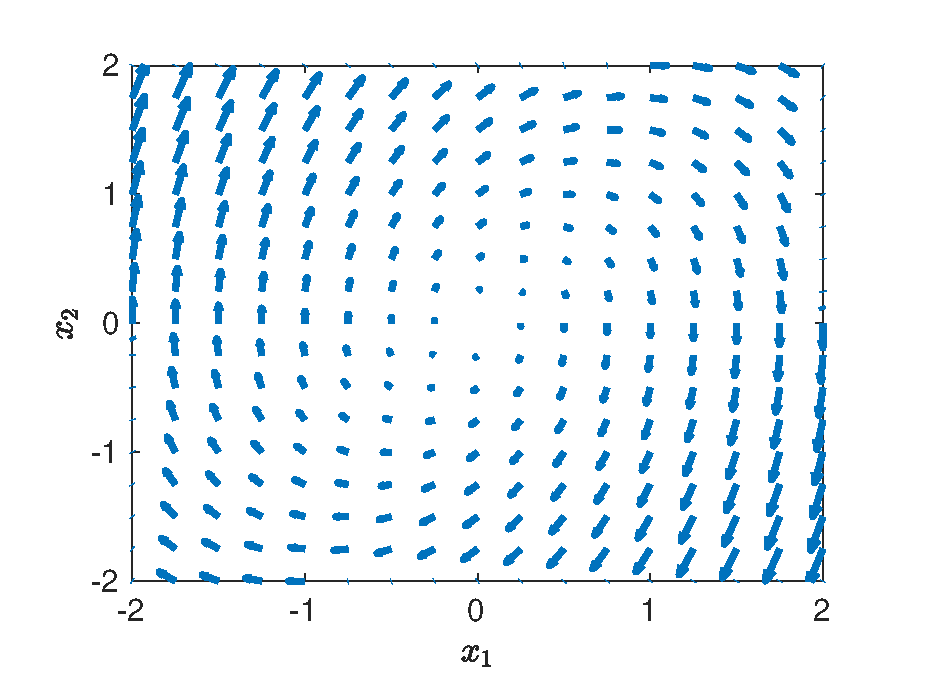
\includegraphics[width = 0.49\columnwidth]{quiver2.eps}
	\label{subfig:sys2_quiver}}
	\subfloat[]{
	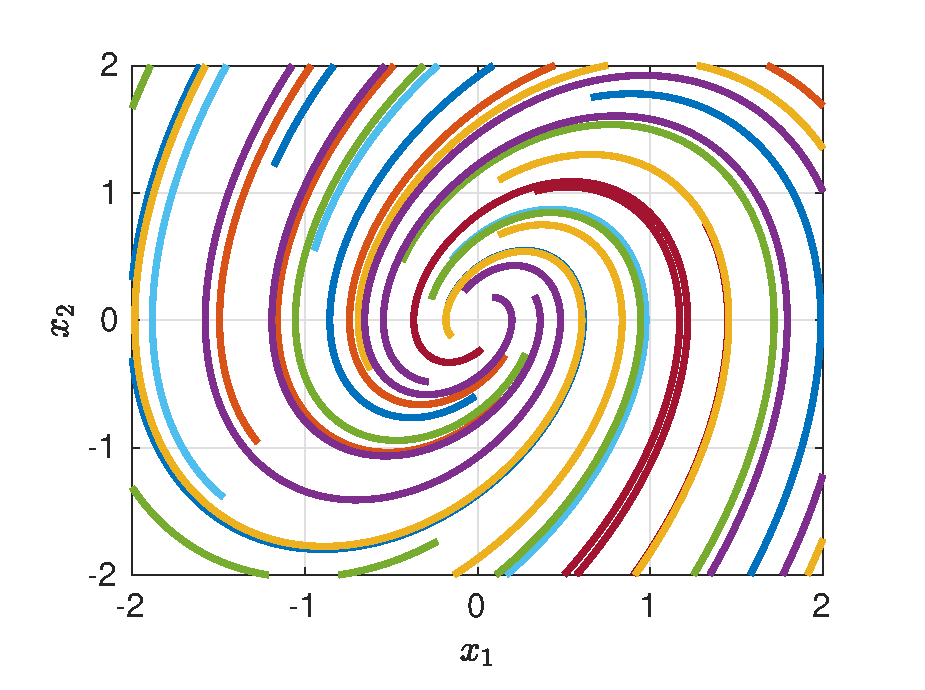
\includegraphics[width = 0.49\columnwidth]{quiver_phase_traj.eps}
	\label{subfig:sys2_phasetraj}}
	\caption{Plan~\subref{subfig:sys2_quiver} et trajectoires~\subref{subfig:sys2_phasetraj} de phase du système~\eqref{eq-chap4:expl linear system VSS 2}.}
	\label{fig:sys2}
\end{figure}
\begin{figure}
	\centering
	\subfloat[]{
	\includegraphics[width = 0.49\columnwidth]{VSS_m.eps}
	\label{subfig:VSS1_quiver}}
	\subfloat[]{
	\includegraphics[width = 0.49\columnwidth]{VSS1_phase_traj2.eps}
	\label{subfig:VSS1_phasetraj}}
	\caption{Plan~\subref{subfig:VSS1_quiver} et trajectoires~\subref{subfig:VSS1_phasetraj} de phase du système~\eqref{eq-chap4:variable struc sys}. La droite  rouge représente la droite $S_1=x_2 + |\lambda_1|x_1=0$, avec $\lambda_1$ est la valeur propre stable de $\matriceA_{\rm BF 1}$ dans~\eqref{eq-chap4:eigen vaues sys1}.}
	\label{fig:VSS1}
\end{figure}
\begin{figure}
	\centering
	\subfloat[]{
	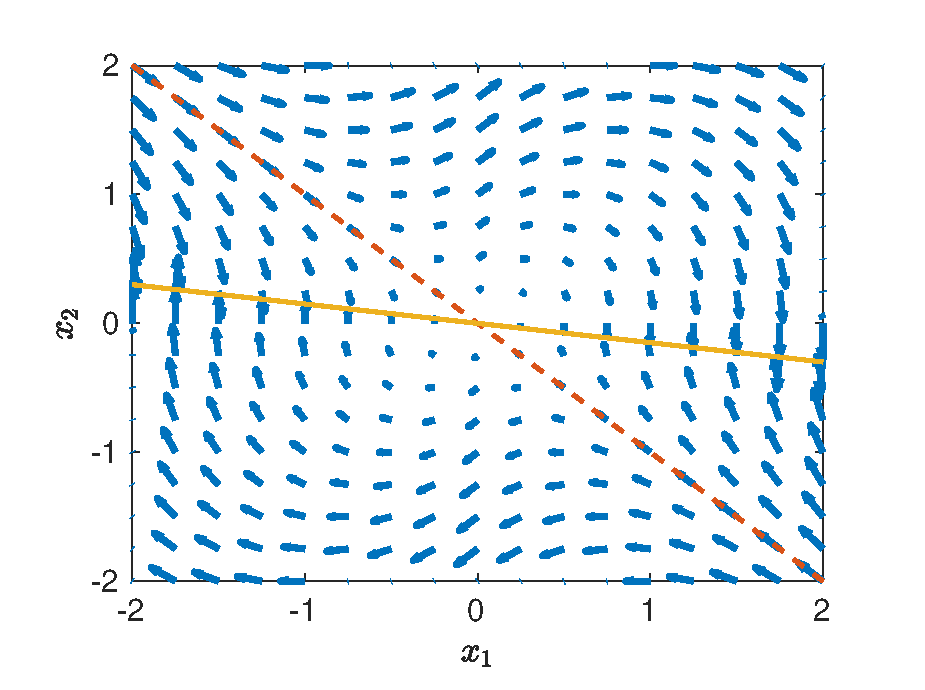
\includegraphics[width = 0.49\columnwidth]{VSS2_m.eps}
	\label{subfig:VSS2_quiver}}
	\subfloat[]{
	\includegraphics[width = 0.49\columnwidth]{VSS2_phase_traj2.eps}
	\label{subfig:VSS2_phasetraj}}
	\caption{Plan~\subref{subfig:VSS2_quiver} et trajectoires~\subref{subfig:VSS2_phasetraj} de phase du système~\eqref{eq-chap4:variable struc sys}. La droite rouge en pointillé représente la droite $S_1=x_2 + |\lambda_1|x_1=0$, avec $\lambda_1$ est la valeur propre stable de $\matriceA_{\rm BF 1}$ dans~\eqref{eq-chap4:eigen vaues sys1}, la droite  jaune représente la droite $S_2=x_2 + cx_1=0$ avec $0<c<|\lambda_1|$.}
	\label{fig:VSS2}
\end{figure}
%\begin{figure}
%	\centering
%	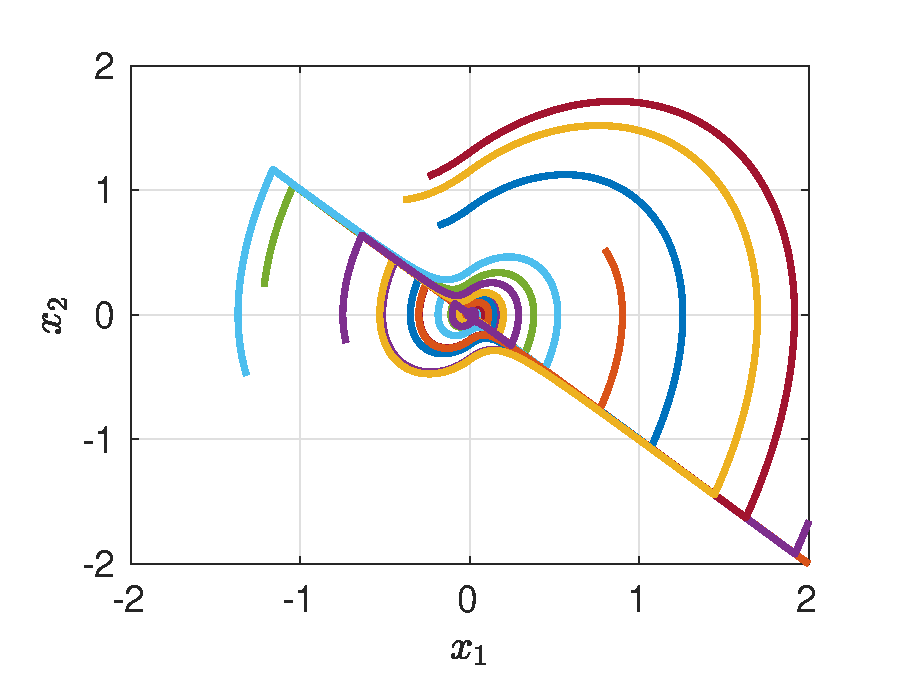
\includegraphics[width = 0.6\columnwidth]{VSS1_phase_traj.eps}
%	\caption{Plan de phase du système~\eqref{eq-chap4:expl linear system VSS 1}. Les droites   jaune et rouge représentent les vecteurs propres relative au valeurs propres $\lambda_1$ et $\lambda_2$ de $\matriceA_{\rm BF 1}$, respectivement.}
%	\label{fig:VSS1 phase traj}
%\end{figure}
%\begin{figure}
%	\centering
%	\includegraphics[width = 0.6\columnwidth]{VSS2_phase_traj.eps}
%	\caption{Plan de phase du système~\eqref{eq-chap4:expl linear system VSS 1}. Les droites   jaune et rouge représentent les vecteurs propres relative au valeurs propres $\lambda_1$ et $\lambda_2$ de $\matriceA_{\rm BF 1}$, respectivement.}
%	\label{fig:VSS2 phase traj}
%\end{figure}
%\begin{itemize}
%	\item Combiner les avantages de chaque système,
%	\item Bénéficier de nouvelles propriétés qui sont absentes dans chacun des systèmes. 
%\end{itemize}